\documentclass{beamer}
	\title{La mia prima presentazione}
	\author{Antonio Michele Miti}
	\date{20 novembre 2015}


%Common symbols
%Common math symbols
	%Number fields
		\newcommand{\Real}{\mathbb{R}}
		\newcommand{\Natural}{\mathbb{N}}
		\newcommand{\Relative}{\mathbb{Z}}
		\newcommand{\Rational}{\mathbb{Q}}
		\newcommand{\Complex}{\mathbb{C}}
	
%equality lingo
	%must be equal
		\newcommand{\mbeq}{\overset{!}{=}} 

% function
	%Domain
		\newcommand{\dom}{\mathrm{dom}}
	%Range
		\newcommand{\ran}{\mathrm{ran}}
	

% Set Theory
	% Power set (insieme delle parti
		\newcommand{\PowerSet}{\mathcal{P}}

%Differential Geometry
	% Atlas
		\newcommand{\Atlas}{\mathcal{A}}
	%support
		\newcommand{\supp}{\textrm{supp}}

	
	
%Category Theory
	%Mor set http://ncatlab.org/nlab/show/morphism
%		\newcommand{\hom}{\textrm{hom}}

%Geometric Lagrangian Mechanics
	% Kinematic Configurations
		\newcommand{\Conf}{\mathtt{C}}
	%Solutions Space
		\newcommand{\Sol}{\mathtt{Sol}}
	%Lagrangian class
		\newcommand{\Lag}{\mathsf{Lag}}
	%Lagrangiana
		\newcommand{\Lagrangian}{\mathcal{L}}
	%Data
		\newcommand{\Data}{\mathsf{Data}}
	%unique solution map
		\newcommand{\SolMap}{\mathbf{s}}
	%Classical Observables
		\newcommand{\Obs}{\mathcal{E}}	
	%Phase Space
		\newcommand{\Phase}{\mathcal{M}}	

		\
		
%Peierls (per non sbagliare più)
		\newcommand{\Pei}{Peierls}
%---------------------------------------------------------------------------------------------------------------------------------------------------------------------

\begin{document}


%\/\/\/\/\/\/\/\/\/\/\/\/\/\/\/\/\/\/\/\/\/\/\/\/\/\/\/\/\/\/\/\/\/\/\/\/\/\/\/\/\/\/\/\/\/\/\/\/\/\/\/\/\/\/\/\/\/\/\/\/\/\/\/\/\/\/\/\/\/
%				Intro
%\/\/\/\/\/\/\/\/\/\/\/\/\/\/\/\/\/\/\/\/\/\/\/\/\/\/\/\/\/\/\/\/\/\/\/\/\/\/\/\/\/\/\/\/\/\/\/\/\/\/\/\/\/\/\/\/\/\/\/\/\/\/\/\/\/\/\/\/\/
	\begin{frame} %Titolo
		\maketitle
	\end{frame}
	
	\begin{frame} % Organizzazione della Presentazione
		\frametitle{Intro}
		(struttura della tesi vs struttura della presentazione)
	\end{frame}
	

%\/\/\/\/\/\/\/\/\/\/\/\/\/\/\/\/\/\/\/\/\/\/\/\/\/\/\/\/\/\/\/\/\/\/\/\/\/\/\/\/\/\/\/\/\/\/\/\/\/\/\/\/\/\/\/\/\/\/\/\/\/\/\/\/\/\/\/\/\/
%				Parte 1 : 	"Foundations of Mechanics"
%\/\/\/\/\/\/\/\/\/\/\/\/\/\/\/\/\/\/\/\/\/\/\/\/\/\/\/\/\/\/\/\/\/\/\/\/\/\/\/\/\/\/\/\/\/\/\/\/\/\/\/\/\/\/\/\/\/\/\/\/\/\/\/\/\/\/\/\/\/		
	\part{Meccanica Geometrica}
		\frame{\partpage}
	
		\begin{frame}
		\frametitle{IDEA Meccanica Geometrica:}
			\begin{itemize}
				\item<1-> Raccontare l'approccio canonico coordinate free alla meccanica classica a finiti gradi
					\begin{itemize}
						\item Lo spazio delle fasi
						\item La forma simplettica
						\item lagrangiana hamiltoniana legendre
						\item struttura di Poisson
					\end{itemize}
				\item<1-> Dire che un suo aspetto importante è che funge da base per le teorie di quantizzazione
				\item<1-> Ci interessa quantizzare i campi quindi ci interessa il formalismo canonico per i campi
				\item<2-> Presentare l'approccio al formalismo canonico dei campi in 2 step:
				\item<3-> Ok, fin qui abbiamo un insieme. Come lo doto di una struttura simplettica?
			\end{itemize}
	\end{frame}
	
	\begin{frame}
		\frametitle{Formalismo canonico}
  			\begin{columns}[T]
    			\begin{column}{.5\textwidth}
     				\begin{block}{Your textblock}
						% Your text here
						(usual approach) I passi principali per la costruzione del formalismo canonico per teorie con $N$ gradi di libertà
						\begin{enumerate}
							\item si introducono la coordinate di configuazione $q^j$ e i momenti canonici coniugati $p^j$
							\item si definisce la 2-forma $\omega = dp^i \wedge dq^i$
							\item combinando $p^i,q^j$ in un'unica variablie $Q^I , I = 1,\ldots,2N$, con $Q^i=p^i$ per $i\leq\leq N$ e $Q^i= q^{i-N}$ per $i>N$. E' possibile riguardare $\omega$ come una matrice $2N \times N$  antisimmetrica i cui elementi non nulli sono
								\begin{displaymath}
									\omega_{i , i+N} = -\omega_{i+N,i} = 1
								\end{displaymath}
							\item le parentesi di poisson per 2 funzioni $A(Q^I) , B(Q^J)$ vengono definite come:
								\begin{displaymath}
									\left[ A , B \right] = \omega^{I J} \frac{\partial A}{\partial Q^I} \frac{\partial B}{\partial Q^J}					
								\end{displaymath}
						\end{enumerate}
    				\end{block}
    			\end{column}
    		   	\begin{column}{.5\textwidth}
			    	\begin{block}{Your image}
						% Your image included here
						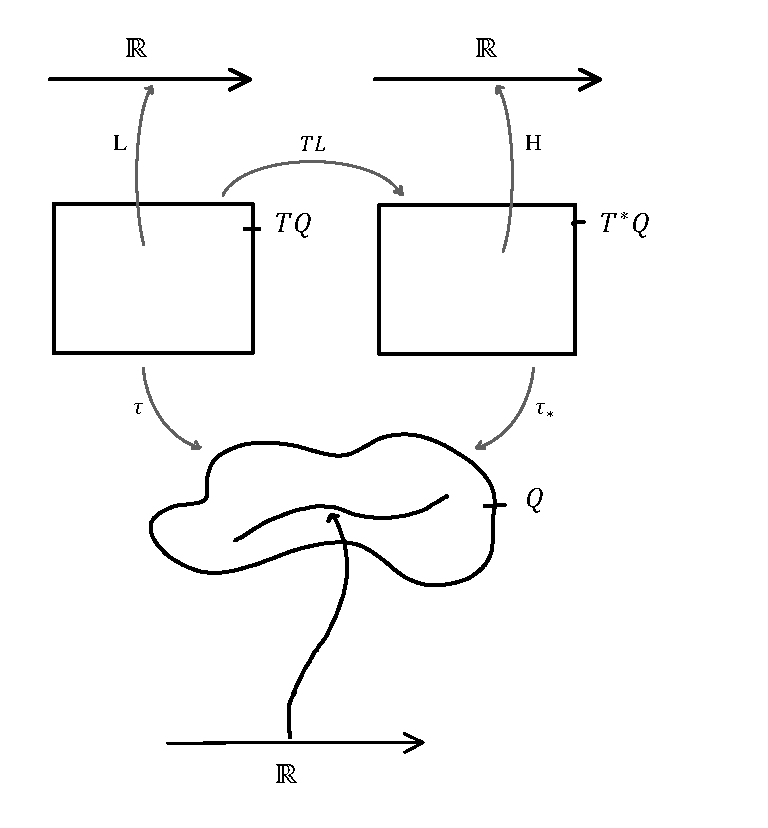
\includegraphics[width=\textwidth]{Presentazione/GeoMecFrameA} 
    				\end{block}
    			\end{column}
  			\end{columns}	
		\end{frame}
		
		\begin{frame}
			\frametitle{Formalismo Canonico Covariante}
  			\begin{columns}[T]
    			\begin{column}{.5\textwidth}
     				\begin{block}{Your textblock}
						% Your text here
						Passaggio Canonico Ordinario a Canonico Covariante (a finiti gradi)
						\\
						Parlare di Conf Sol e S
    				\end{block}
    			\end{column}
    		   	\begin{column}{.5\textwidth}
			    	\begin{block}{Your image}
						% Your image included here
						\includegraphics<1> [width=\textwidth]{Presentazione/GeoMecFrameA} 
						\includegraphics<2> [width=\textwidth]{Presentazione/GeoMecFrameB} 
						\includegraphics<3>[width=\textwidth]{Presentazione/GeoMecFrameC} 
    				\end{block}
    			\end{column}
  			\end{columns}		
		\end{frame}
	
		\begin{frame}
			\frametitle{Formalismo Covariante esteso}
  			\begin{columns}[T]
    			\begin{column}{.5\textwidth}
     				\begin{block}{Your textblock}
						% Your text here
						Il formalismo covariante si estende facilmente a sistemi più generali! ad esempio  i campi intesi come sistemi fisici con un set continuo di gradi \\
						Passaggio Canonico Covariante a Finiti Gradi a Canonico Covarianti a gradi continuo \\
						Parlare di Conf Sol e S	per i campi, notare che la definizione della lagrangiana è più delicate
    				\end{block}
    			\end{column}
    		   	\begin{column}{.5\textwidth}
			    	\begin{block}{Your image}
						% Your image included here
						\includegraphics<1> [width=\textwidth]{Pictures/FieMecFrame} 
						\includegraphics<2> [width=\textwidth]{Pictures/AbstractFieldTheory} 
    				\end{block}
    			\end{column}
  			\end{columns}		


		\end{frame}
		
		\begin{frame}
			\frametitle{Recuperare il formalismo canonico non covariante}		
			(extra) Recupare il formalismo canonico non covariante anche per i campi costruendo il dato su una superficie di Cauchy (ricordare che al continuo ci sono controesempi che darboux non vale)
			\\
			Lo si fa per sistemi su spazitempi globalmenente iperbolici. in breve sono varietà molto generali in cui è possibile definire per bene i problemi di cauchy
		\end{frame}

		\begin{frame}
			\frametitle{A che punto siamo?}		
			Fin qui abbiamo degli spazi canditati ad essere lo spazio delle fasi.
			Ciò che manca è la loro dotazione di una forma simplettica o di un algebra di Poisson di osservabili.

		\end{frame}


%\/\/\/\/\/\/\/\/\/\/\/\/\/\/\/\/\/\/\/\/\/\/\/\/\/\/\/\/\/\/\/\/\/\/\/\/\/\/\/\/\/\/\/\/\/\/\/\/\/\/\/\/\/\/\/\/\/\/\/\/\/\/\/\/\/\/\/\/\/
%				Parte 2 : 	"L'algoritmo di Peierls"
%\/\/\/\/\/\/\/\/\/\/\/\/\/\/\/\/\/\/\/\/\/\/\/\/\/\/\/\/\/\/\/\/\/\/\/\/\/\/\/\/\/\/\/\/\/\/\/\/\/\/\/\/\/\/\/\/\/\/\/\/\/\/\/\/\/\/\/\/\/		
	\part{Costruzione della struttura simplettica nel caso dei campi classici}
	\frame{\partpage}
	
	\begin{frame}
		\frametitle{Cappello sul Metodo di Peierls }
			\begin{itemize}
				\item semplificare: usare i grafici già fatti e considerare solo i campi scalari
			\end{itemize}
			His essential insight was to consider the advanced and retarded “effect of one quantity (A) on another (B).” Here, A and B are to
be functions on H. 

			The advanced  and retarded  effects of A on B are then defined by comparing the original system with a new system defined by the action $S_\epsilon = S + \epsilon A$ and the same space H of histories. 
			Under retarded (advanced) boundary conditions for which the solutions $\phi \in S$ and $\phi_\epsilon	\in S_\epsilon$ coincide to the past (future) of the support of A, the quantity $B_0 = B(\phi)$ computed using $\phi$ will in general differ from $B_\epsilon = B(\phi_\epsilon)$ computed using $\phi_\epsilon$.
			For small epsilon, the difference between these quantities defines the retarded (advanced) effect of A on B through:
which depends on the unperturbed solution $\phi$.
	\end{frame}
	
	\begin{frame}
		\frametitle{I passi del metodo di Peierls}
		The procedure can be summarized in a few steps:
	\begin{enumerate}
		\item Consider a \emph{disturbance} $\chi$ that is a time-compact Lagrangian density .
		\item Construct the \emph{perturbation of a solution under the action of $\chi$}.
		%\emph{perturbation of a solution under the disturbance}. (correzione CD
		\item Define the \emph{effect of the disturbance} on a second Lagrangian functional.
		\item Assemble the mutual effects of two different Lagrangian densities to give a \emph{brackets}.
	\end{enumerate}	
	\end{frame}
	
	\begin{frame}
		\frametitle{ Concetto chiave dell'algoritmo di peierls}
		Sono le \emph{disturbance lagrangiane}
		
	\end{frame}
	
	\begin{frame}
		\frametitle{Applicabilità del metodo di Peierls}	
			The Peierls' construction algorithm is well defined for a specific class of systems:
		\begin{enumerate}[A)]
			\item\label{HpPeierls1} Linear field theory: $E=(E,\pi,M;Q)$ is a vector bundle.
			%\item  Lagragian dynamics: $P=Q_\Lagrangian$ is a L.P.D.O.
			\item\label{HpPeierls2} $P=Q_\Lagrangian$ is a Green-hyperbolic linear partial differential operator.
			\item\label{HpPeierls3} $M$ is a globally hyperbolic spacetime.
			%\item Motion operator $P$ is a Green-hyperbolic.
		\end{enumerate}	
	\end{frame}
	
	\begin{frame}
		\frametitle{Peierls non è l'unica soluzione}
		Ci sono altri metodi provati essere equivalenti a peierls
	
	\end{frame}
	
	
%\/\/\/\/\/\/\/\/\/\/\/\/\/\/\/\/\/\/\/\/\/\/\/\/\/\/\/\/\/\/\/\/\/\/\/\/\/\/\/\/\/\/\/\/\/\/\/\/\/\/\/\/\/\/\/\/\/\/\/\/\/\/\/\/\/\/\/\/\/
%				Parte 3 : 	"Realizzazione Specifica del campo di Jacobi"
%\/\/\/\/\/\/\/\/\/\/\/\/\/\/\/\/\/\/\/\/\/\/\/\/\/\/\/\/\/\/\/\/\/\/\/\/\/\/\/\/\/\/\/\/\/\/\/\/\/\/\/\/\/\/\/\/\/\/\/\/\/\/\/\/\/\/\/\/\/		
	\part{Realizzazione per il Caso specifico dei campi di Jacobi}
	\frame{\partpage}

	\begin{frame}
		\frametitle{ IDEA }
			\begin{itemize}
				\item ricordare le basi, varietà riemmaniana, metrica ,geodetiche jacobi
			\end{itemize}
	\end{frame}


%\/\/\/\/\/\/\/\/\/\/\/\/\/\/\/\/\/\/\/\/\/\/\/\/\/\/\/\/\/\/\/\/\/\/\/\/\/\/\/\/\/\/\/\/\/\/\/\/\/\/\/\/\/\/\/\/\/\/\/\/\/\/\/\/\/\/\/\/\/
%				Fine	!!!
%\/\/\/\/\/\/\/\/\/\/\/\/\/\/\/\/\/\/\/\/\/\/\/\/\/\/\/\/\/\/\/\/\/\/\/\/\/\/\/\/\/\/\/\/\/\/\/\/\/\/\/\/\/\/\/\/\/\/\/\/\/\/\/\/\/\/\/\/\/		
	\begin{frame}
		\frametitle{ Conclusioni }
			\begin{itemize}
				\item Interpretazione geometrica: punto chiave: ci sono 2 spazi la cui geometria soggiace al discorso: spazio delle soluzioni e spazio delle lagrangiane
			\end{itemize}
	\end{frame}
	
\end{document}


		\begin{enumerate}
			\item si introducono la coordinate di configuazione $q^j$ e i momenti canonici coniugati $p^j$
			\item si definisce la 2-forma $\omega = dp^i \wedge dq^i$
			\item combinando $p^i,q^j$ in un'unica variablie $Q^I , I = 1,\ldots,2N$, con $Q^i=p^i$ per $i\leq\leq N$ e $Q^i= q^{i-N}$ per $i>N$. E' possibile riguardare $\omega$ come una matrice $2N\times \N$ antisimmetrica i cui elementi non nulli sono
				\begin{displaymath}
					\omega_{i , i+N} = -\omega_{i+N,i} = 1
				\end{displaymath}
			\item le parentesi di poisson per 2 funzioni $A(Q^I) , B(Q^J)$ vengono definite come:
				\begin{displaymath}
						\left[ A , B \right] = \omega^{I J} \frac{partial A}{\partial Q^I} \frac{\partial B}{\partial Q^J}					
				\end{displaymath}
		\end{enumerate}